\documentclass{beamer}


%\usetheme{Copenhagen}
\usetheme{CambridgeUS}
%\usetheme{madrid}
\usecolortheme{dolphin}
\usecolortheme{orchid}
\usepackage[utf8]{inputenc}
%\usepackage[ngerman]{babel}
\usepackage{amsmath}
\usepackage{lmodern}
%\usepackage{marvosym}
\usepackage{enumerate}
\usepackage{pgfplots}
\usepackage{textcomp}
\usepackage{fancyhdr}
\usepackage{amsthm}
\usepackage{amsfonts}
\usepackage{graphicx} % Allows including images
\usepackage{booktabs} % Allows the use of \toprule, \midrule and \bottomrule in tables
\usepackage{braket}
\usepackage{mathabx}
\usepackage{physics}
\usepackage{subfigure}
\renewcommand{\va}[1]{\vec{#1}}
\usepackage{todonotes}
\let\todox\todo
\renewcommand\todo[1]{\todox[inline]{#1}}
%
%\usepackage{tikz}

\usepackage[backend=bibtex8,sorting=none]{biblatex}
\addbibresource{refs.bib}

\newcommand{\upd}[1]{^\mathrm{#1}}
\newcommand{\ind}[1]{_\mathrm{#1}}


%----------------------------------------------------------------------------------------
%	TITLE PAGE
%----------------------------------------------------------------------------------------

\title[Hawking Radiation for Observers]{\vspace{1cm}Hawking Radiation as Seen by Observers\\\small{Bachelor thesis}}

\author[Friedrich Hübner]{Friedrich Hübner\\Universität Bonn}
\date{07.09.2018}

\begin{document}
\beamertemplatenavigationsymbolsempty
\titlepage

\begin{frame}{Introduction}
\begin{itemize}
	\item Hawking 1974 \cite{hawking}: black holes radiate at \(T\ind{H} = \frac{1}{8\pi M}\)
	\item[]
	\item Minkowski space:
		\begin{itemize}
			\item Inertial observer: no particles
			\item Accelerating observer: heat bath (Unruh effect)
		\end{itemize}		 
	\item[]
	\item Observers around the black hole:
		\begin{itemize}
			\item Freely falling (e.g. orbiting): no particles?
			\item Static observer: heat bath?
		\end{itemize}
\end{itemize}
\end{frame}

\frame{\setcounter{tocdepth}{1}\hspace{1cm}\tableofcontents}

\section{QFT in curved spacetime}
\subsection{Scalar field}
\begin{frame}{Massless scalar field in curved spacetime\cite{davies}}
\begin{itemize}
	\item Spacetime metric: \(g_{\mu\nu}\)
	\item Lagrangian: \(\mathcal{L} = -\frac{1}{2}\sqrt{|g|} g^{\mu\nu} \partial_\mu \phi\,\partial_\nu \phi\)
	\item Klein-Gordon equation: \(\nabla_\mu\nabla^\mu \phi = 0\)
	\item Scalar product: \((\phi|\psi) := i \int_{\Sigma}\dd{S^\mu} \phi^*\nabla_\mu \psi - \psi\nabla_\mu \phi^*\)
	\item Orthonormal basis: \((u_i|u_j) = \delta_{ij},\;(u_i|u_j^*) = 0,\;(u_i^*|u_j^*) = -\delta_{ij}\)
	\item Quantisation: \(\phi(\vb{x}) = \sum_i u_i a_i + u_i^*a_i^\dagger\)
\end{itemize}
\end{frame}

\begin{frame}{State of the QFT\cite{davies}}
\begin{itemize}
	\item Vacuum: \(a_i \ket*{0} = 0\)
	\item Problem: \(u_i \to v_j, a_i \to b_j\): \(b_i \ket*{0} \neq 0\)
	\item[] \(\to\) Need to guess state!
	\item Static spacetime: choose vacuum w.r.t. positive frequency modes: \(u_i \sim e^{-i\omega t}\)
	\item What does an observer see? 
\end{itemize}
\end{frame}

\begin{frame}{Wightman function\cite{davies}}
\begin{itemize}
	\item Vacuum Wightman function: 
	\begin{itemize}
		\item \(D^+(\vb{x},\vb{x}') := \bra*{0}\phi(\vb{x})\phi(\vb{x}')\ket*{0}\)
		\item \(D^+(\vb{x},\vb{x}') = \sum_i u_i(\vb{x}) u_i^*(\vb{x}')\)
		\item \(\nabla_\mu\nabla^\mu D^+(\vb{x},\vb{x}') = 0\)
	\end{itemize}
	\item[]
	\item Thermal Wightman function:
	\begin{itemize}
		\item Replace \(\bra*{0}\dots\ket*{0}\) by \(\frac{1}{Z} \mathrm{Tr}\,e^{-\beta H} \dots\)
		\item If \(D^+\) real: \(D^+_\beta(t,\va{x};t',\va{x}') = \sum_n D^+(t-i\beta n, \va{x};t',\va{x}')\)
	\end{itemize}
\end{itemize}
\end{frame}

\subsection{Unruh detector}
\begin{frame}{Unruh detector\cite{davies}}
\begin{itemize}
	\item Detector model: \(\mathcal{H}\ind{detector} = c \cdot m(\tau)\cdot \phi(\vb{x}(\tau))\),\, \(c \ll 1\)
\end{itemize}
\begin{block}{Transition rate}
\(\dv{F_E}{\tau} = 2 \mathrm{Re}\,\int_{-\infty}^0 \dd{\tau'} e^{-i E \tau'} D^+(\vb{x}(\tau + \tau'), \vb{x}(\tau))\)
\end{block}
\begin{block}{Constant rate}
\(\dv{F_E}{\tau} = \int_{-\infty}^\infty \dd{\tau} e^{-i E \tau} D^+(\vb{x}(\tau), \vb{x}(0))\)
\end{block}
\begin{itemize}
	\item Interpretation: \(F_E\) is particle population for observer 
\end{itemize}
\end{frame}
\subsection{Minkowski space}
\begin{frame}{Minkowski space\cite{davies}}
\begin{itemize}
	\item Wightman function: \(D^+(\vb{x},\vb{x}') = -\frac{1}{4\pi^2} \frac{1}{(t-t'-i\varepsilon)^2 - |\va{x}-\va{x}'|^2}\)
	\item Static observer: \(t(\tau) = \tau, \va{x}(\tau) = \mathrm{const}\)
	\begin{itemize}
		\item \(D^+(\vb{x}(\tau),\vb{x}(0)) = -\frac{1}{4\pi^2} \frac{1}{(\tau-i\varepsilon)^2}\)
		\item Fourier transform: \(\dv{F_E}{\tau} = 0\)
	\end{itemize}
	\item[]\(\to\) Inertial observer: vacuum contains no particles
\end{itemize}
\begin{figure}
\centering
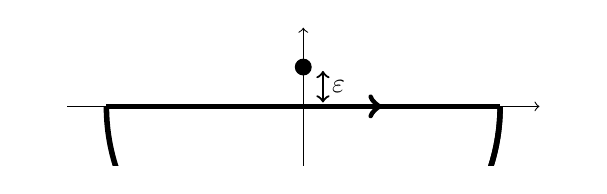
\begin{tikzpicture}[scale=0.5]
  \clip (-7,2) rectangle (7,-1.5);
  \draw[->] (-6,0) -- (6,0);
  \draw[->] (0,-5.5) -- (0,2);
  \draw[line width=2] (-5,0) -- (5,0);
  \draw[line width=2,->] (-5,0) -- (2,0);
  \draw[line width=2] (5,0) arc (0:-180:5);
  \draw[line width=2,->] (5,0) arc (0:-135:5);
  \draw[fill=black] (0,1) circle (0.2);
  \draw[thick,<->] (0.5,0.1) -- (0.5,0.9);
  \node at (0.9,0.5) {$\varepsilon$};
\end{tikzpicture}
\caption{Pole structure}
\end{figure}
\end{frame}

\begin{frame}{Unruh effect\cite{davies}}
\begin{itemize}
	\item Accelerating observer: \(t(\tau) = 1/\alpha \sinh \alpha\tau,\,x(\tau) = 1/\alpha \cosh \alpha\tau\)
	\begin{itemize}
		\item \(D^+(\vb{x}(\tau), \vb{x}(\tau')) = -\frac{\alpha^2}{16\pi^2} \frac{1}{\sinh^2\frac{\alpha(\tau-\tau')}{2}}\)
	\end{itemize}
	\item Thermal state: \(D^+_\beta(\vb{x},\vb{x}') = -\frac{1}{4\beta^2} \frac{1}{\sinh[2](\frac{\pi}{\beta}\sqrt{(t-t'-i\varepsilon)^2 - |\va{x}-\va{x}'|^2})}\)
	\begin{itemize}
		\item Static observer: \(D^+_\beta(\vb{x}(\tau),\vb{x}(\tau')) = -\frac{1}{4\beta^2} \frac{1}{\sinh[2](\frac{\pi}{\beta} (\tau-\tau'))}\)
	\end{itemize}
	\item Set \(\beta = 2\pi/\alpha\)
	\item Accelerating observer: vacuum is a thermal state
\end{itemize}
\end{frame}

\frame{\setcounter{tocdepth}{1}\hspace{1cm}\tableofcontents}

\section{Static spacetimes and equivalence principle}
\begin{frame}{Static spactimes}
\begin{itemize}
	\item Metric: \(\dd{s^2} = -\beta(\va{x}) \dd{t^2} + g_{ij}(\va{x}) \dd{x^i} \dd{x^j}\)
	\item[]
	\item Positive frequency solutions: \(u_{i}(t, \va{x}) = \frac{1}{\sqrt{2\omega_i}}e^{-i\omega_i t} A_i(\va{x})\)
	\item[]
	\item State of QFT -- vacuum: \(a_i \ket*{0} = 0\)
\end{itemize}
\end{frame}

\subsection{Properties of the Wightman function}
\begin{frame}{Properties of Wightman function}
\begin{block}{Wightman function in normal coordinates}
\(D^+(\vb{x},0) = -\frac{1}{4\pi^2} \frac{1}{a(t-i\varepsilon)^2 - |\va{x}|^2} + \order{x^2}\hspace{3cm} a = \beta(0)\)
\end{block}
\begin{itemize}
	\item \(D^+\) has second order pole at \(\vb{x} = 0\)
	\item \(\varepsilon\) shifts pole to upper half
	\item[] \(\to\) drop pole at \(\vb{x} = 0\)
	\item[]
	\item No more singularities inside lightcone
	\item \(D^+\) is real inside lightcone
\end{itemize}
\begin{figure}
\centering
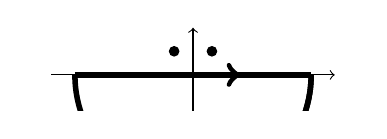
\begin{tikzpicture}[scale=0.3]
  \clip (-7,2) rectangle (7,-1.5);
  \draw[->] (-6,0) -- (6,0);
  \draw[->] (0,-5.5) -- (0,2);
  \draw[line width=2] (-5,0) -- (5,0);
  \draw[line width=2,->] (-5,0) -- (2,0);
  \draw[line width=2] (5,0) arc (0:-180:5);
  \draw[line width=2,->] (5,0) arc (0:-135:5);
  \draw[fill=black] (-0.8,1) circle (0.2);
  \draw[fill=black] (0.8,1) circle (0.2);
  %\draw[thick,<->] (0.5,0.1) -- (0.5,0.9);
  %\node at (0.9,0.5) {$\varepsilon$};
\end{tikzpicture}
\caption{Pole shift}
\end{figure}
\end{frame}


\subsection{Observers}
\subsubsection{Static observer}
\begin{frame}{Static observers}
\begin{block}{Lemma 1}
In a static spacetime a static observer does not observe any particles.
\end{block}
\begin{itemize}
	\item \(t(\tau) = \frac{\tau}{\sqrt{a}}\)
	\item \(u_i~=~\frac{1}{\sqrt{2\omega_i}}e^{-i\omega_i t} A_i(\va{x})\)
	\item \(D^+(\vb{x}(\tau), \vb{x}(0)) = \sum_i \frac{1}{2\omega_i} e^{-i\omega_i\tau/\sqrt{a}} A_i(\va{x}_0)A_i^*(\va{x}_0)\)
	\begin{align*}
	\dv{F_E}{\tau} &= \sum_i \frac{1}{2\omega_i} A_i(\va{x}_0)A_i^*(\va{x}_0) \qty(\int_{-\infty}^\infty \dd{\tau} e^{-i E \tau} e^{-i\omega  \tau/\sqrt{a}})\\
	 	&= \sum_i \frac{1}{2\omega_i} A_i(\va{x}_0)A_i^*(\va{x}_0) \delta\qty(E + \omega/\sqrt{a}) = 0
	\end{align*}
\end{itemize}
\end{frame}

\subsubsection{Observers along Killing vectors}
\begin{frame}{Observers along Killing vectors}
\begin{block}{Lemma 2}
An observer moving along a spatial Killing vector \(\vb{k}\) will see excitations if and only if there exists at least one solution \(u\): \(\frac{A}{|B|} < \frac{|m|}{\omega}\).
\begin{itemize}
	\item \(\dot{\vb{x}} = A\partial_t + B\vb{k}\)
	\item \(\vb{k} u = i m\,u, \partial_t u = - i \omega\,u\)
\end{itemize}
\end{block} 
\begin{itemize}
	\item \(u_{m, i} = \tilde{A}_i(y_1, y_2) e^{-i\omega t} e^{i m \xi}\)
	\item Schwarzschild/Minkowski circular orbit: \(\vb{k} = \partial_\varphi\), 
	\begin{itemize}
		\item \(u \sim e^{-i\omega t}e^{i m \varphi}\)\hspace{5cm} \(|m| \in \mathbb{N}, \omega > 0\)
		\item \(\frac{|m|}{\omega}\) unbounded \(\to\) sees particles
	\end{itemize}
	\item Geodesic observers see particles!
\end{itemize}
\end{frame}


\begin{frame}{Equivalence principle?}
\begin{itemize}
	\item Equivalence principle: local effects
	\item[]
	\item Unruh detector: global effect
		\[\dv{F_E}{\tau} = \int_{-\infty}^\infty \dd{\tau} e^{-i E \tau} D^+(\vb{x}(\tau), \vb{x}(0))\]
	\item[]
	\item Depends on whole history of observer 
\end{itemize}
\end{frame}


\subsubsection{General observer}
\begin{frame}{General observers}
\begin{itemize}
	\item Transition rate not constant: \(\dv{F_E}{\tau} = 2 \mathrm{Re}\,\int_{-\infty}^0 \dd{\tau'} e^{-i E \tau'} D^+(\vb{x}(\tau + \tau'), \vb{x}(\tau))\)
	\item[]\(\to\) can not use residuum theorem
	\item How to handle pole at \(\tau' = 0\)?
	\item[]
	\item Expansion: \(D^+(\vb{x}(\tau'), 0) = - \frac{1}{4\pi^2\tau'^2} + W(\tau')\)
	\item \(\frac{1}{\tau'^2}\) term does not contribute
	\item \(W(\tau')\) is non-singular
\end{itemize}
\begin{figure}
\centering
\begin{tikzpicture}[scale=0.5]
  \clip (-7,2) rectangle (7,-1.5);
  \draw[->] (-6,0) -- (6,0);
  \draw[->] (0,-5.5) -- (0,2);
  \draw[line width=2] (-5,0) -- (0,0);
  \draw[line width=2,->] (-6,0) -- (-2,0);
  \draw[fill=black] (0,1) circle (0.2);
  \draw[thick,<->] (0.5,0.1) -- (0.5,0.9);
  \node at (0.9,0.5) {$\varepsilon$};
\end{tikzpicture}
\caption{Pole structure}
\end{figure}
\end{frame}

\frame{\setcounter{tocdepth}{1}\hspace{1cm}\tableofcontents}

\section{Black holes}
\begin{frame}{Black holes}
\begin{itemize}
	\item Consider star
	\item \(\dd s^2 = -f(r)\dd{t^2} + \frac{1}{f(r)}\dd{r^2} + r^2 \dd{\Omega}\) where \(f(r) = 1 - 2M/r\)
	\item QFT in vacuum state
	\item Collapse to black hole: thermal state with \(\beta\ind{H} = 8\pi M\)\cite{hawking}
	\item What spectrum will observers see before and after the collapse?
\end{itemize}
\begin{block}{Vacuum Wightman function}
	\(D^+(\vb{x}, \vb{x}') \approx -\frac{1}{4\pi^2 \sqrt{f(r)f(r')}} \frac{1}{(t-t'-i\varepsilon)^2 - r_*^2 - r_*'^2 + 2r_*r_*' \cos{\alpha}}\) \hspace{1cm} \(r > 200M\)
\end{block}
\begin{itemize}
	\item Tortoise coordinate: \(r_* = r + 2M \ln \frac{r-2M}{2M}\)
\end{itemize}
\end{frame}


\subsection{Circular observer}

\begin{frame}{Circular Observer before collapse}
\begin{itemize}
	\item Circular observer: \(r = \mathrm{const}, t = A\tau, \phi = B \tau\)
	\item[]
	\item \(D^+(\vb{x}(\tau), \vb{x}(\tau')) = -\frac{1}{4\pi^2f(r)} \frac{1}{(A(\tau-\tau')-i\varepsilon)^2 - 2r_*^2 (1 - \cos{B(\tau-\tau')})}\)
	\item[]
	\item Fourier transform: \(\dv{F_E}{\tau} \sim e^{-E/B x_0}\)
\end{itemize}
\end{frame}

\subsection{After collapse}
\begin{frame}{After collapse}
\begin{itemize}
	\item[1.] Find thermal Wightman function
	\item[]
	\item[2.] How to determine observed temperature?
	\item[]
	\item[3.] Apply to different observers:
	\begin{itemize}
		\item Static
		\item Circular geodesic
		\item Infalling geodesic (dropped at infinity, no initial velocity)
	\end{itemize}
\end{itemize}
\end{frame}


\begin{frame}{Thermal Wightman function}

\begin{itemize}
	\item Thermal Wightman function:
	\begin{align*}
		D_\beta^+(t(\tau')) &= \sum_{n=-\infty}^\infty D^+(t(\tau') - i \beta n)\\
			&= \sum_{n=-\infty}^\infty -\frac{1}{4\pi^2 (\tau' - i\beta \sqrt{a} n)^2} + W(\tau'(t - i\beta n))\\
			&= -\frac{1}{4\beta^2 a} \frac{1}{\sinh[2](\frac{\pi}{\beta \sqrt{a}} \tau')} + W_\beta(\tau')
	\end{align*}
	\item Static observers: \(T = \frac{T\ind{H}}{\sqrt{a}}\) (Tolman relation)
	\item General: Corrections from \(W_\beta(\tau')\)
	\begin{itemize}
		\item Temperature shift?
		\item Non thermal?
	\end{itemize}
\end{itemize}
\end{frame}

\begin{frame}{Determining the temperature}
\begin{itemize}
	\item Expect thermal spectrum + non thermal spectrum
	\item Fit temperature: Minimize \(\int_0^\infty \dd{E} \qty|\dv{F_E}{\tau} - \qty(\dv{F_{E}}{\tau})_\beta|^2\)
\end{itemize}
\begin{figure}
\centering
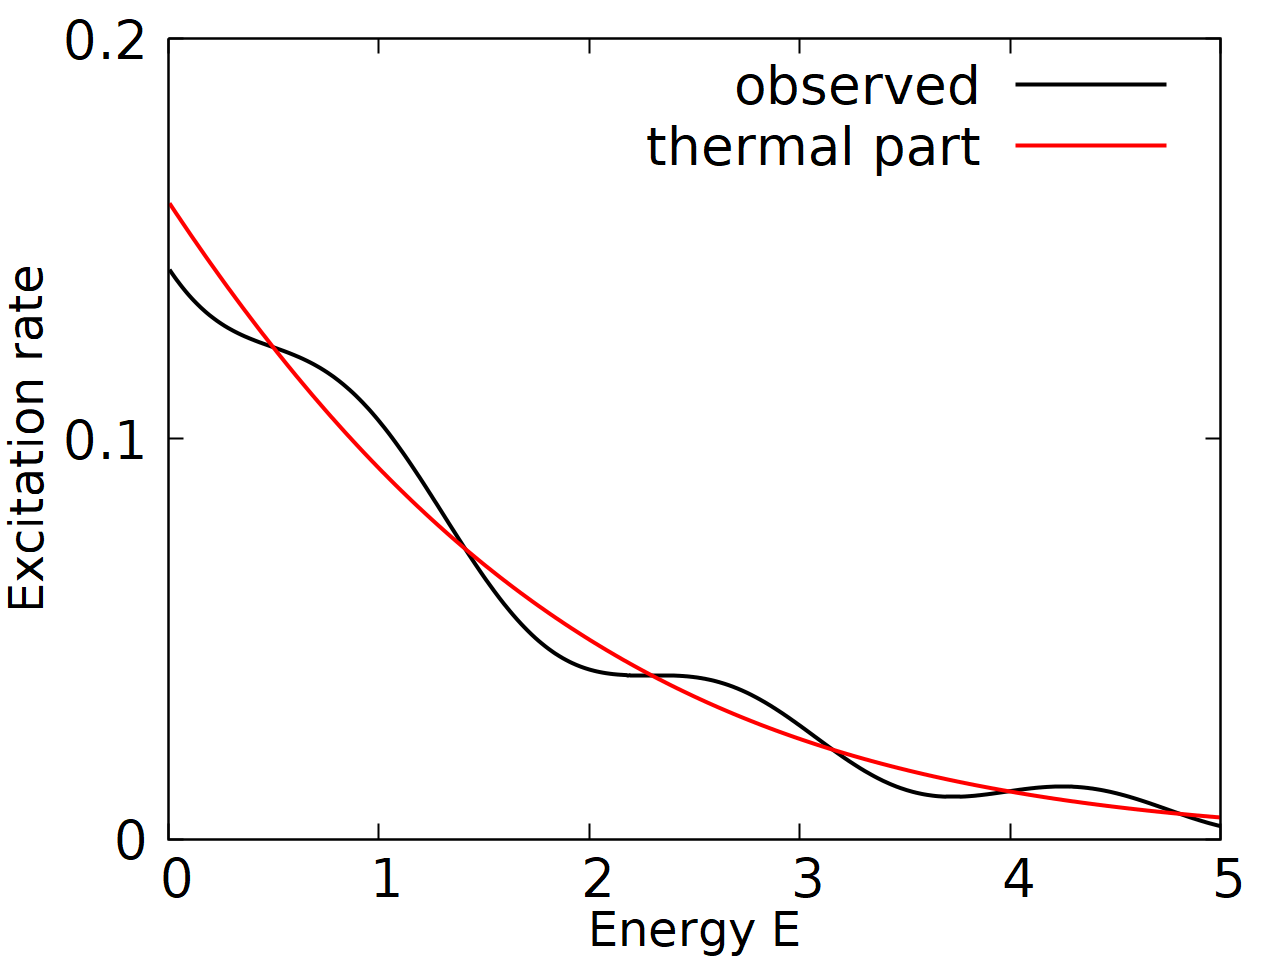
\includegraphics[scale=0.15]{plot/thermal_fit.png}
\caption{Observed and thermal spectrum}
\end{figure}
\end{frame}

\begin{frame}{Determining the temperature}
\begin{itemize}
	\item Minimize instead \(\int_{-\infty}^0 \dd{\tau'} \qty|D^+(\vb{x}(\tau + \tau'), \vb{x}(\tau)) - D_\beta\upd{M}(\tau')|^2\)
	\item[]
	\item Expect small shift: 
	\item[] \(D_\beta\upd{M}(\tau') \approx D_{\beta\ind{H}}\upd{M}(\tau') + \alpha g(\tau')\) where \(\alpha = \frac{\Delta\beta}{\beta\ind{H}} = - \frac{\Delta T}{T\ind{H}}\)
	\item[]
	\item Minimize \(\int_{-\infty}^0 \dd{\tau'} \qty|h(\tau') - \alpha g(\tau')|^2\)\\
	where \(h(\tau') = D^+(\vb{x}(\tau + \tau'), \vb{x}(\tau)) - D_{\beta\ind{H}}\upd{M}(\tau')\)
	\item[]
\end{itemize}
\[\alpha = \frac{\int_{-\infty}^0 \dd{\tau'} h(\tau')\cdot g(\tau')}{\int_{-\infty}^0 \dd{\tau'} g(\tau')^2}\] 
\end{frame}

\subsection{Result}
\begin{frame}{Static observer}
\begin{figure}
	\centering
    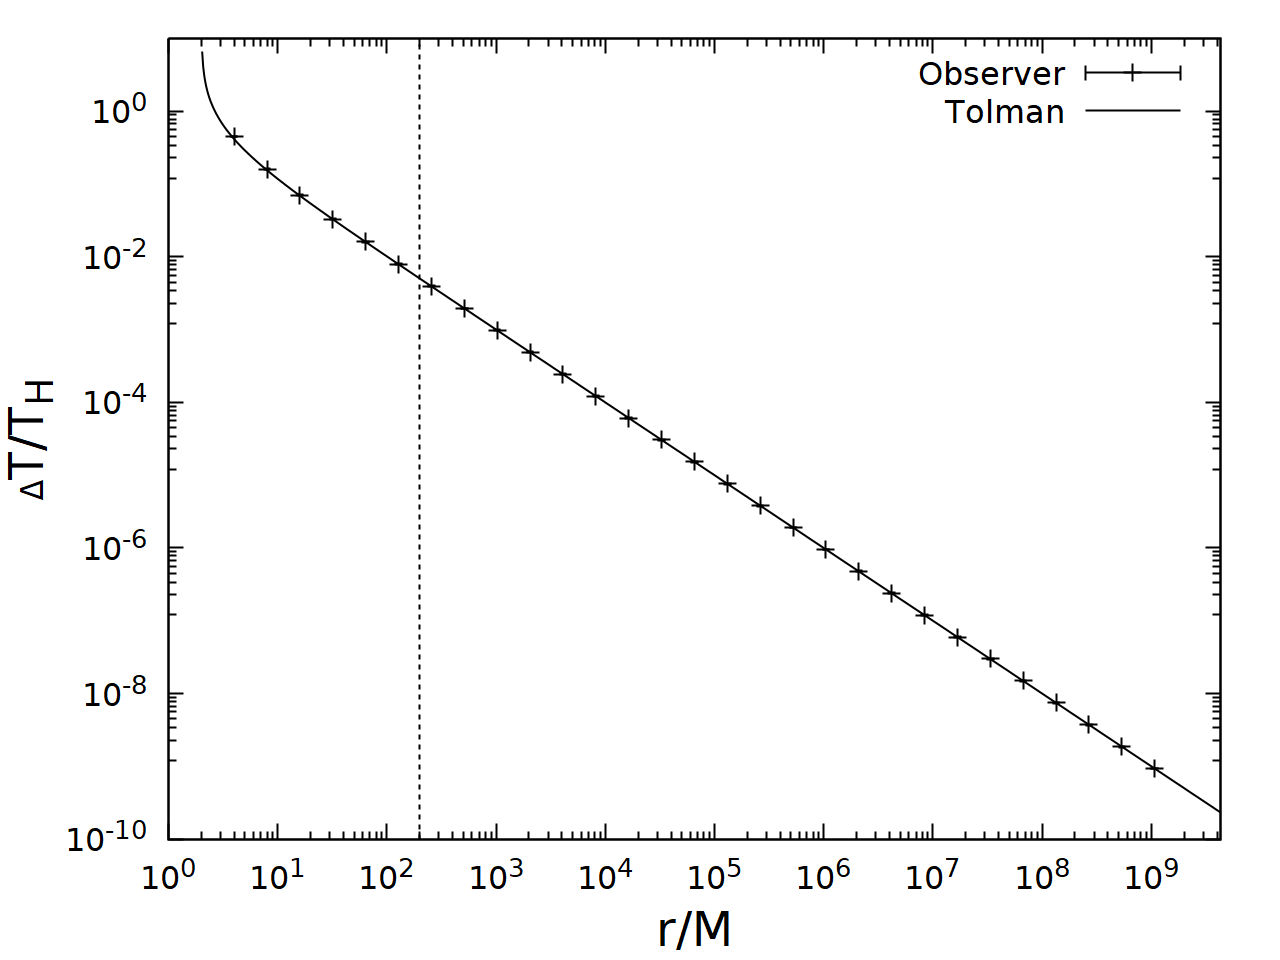
\includegraphics[width=9cm]{../cpp/final/stat.png}
    \caption{Relative temperature shift}
\end{figure}
\end{frame}

\begin{frame}{Static observer}
\begin{figure}
	\centering
    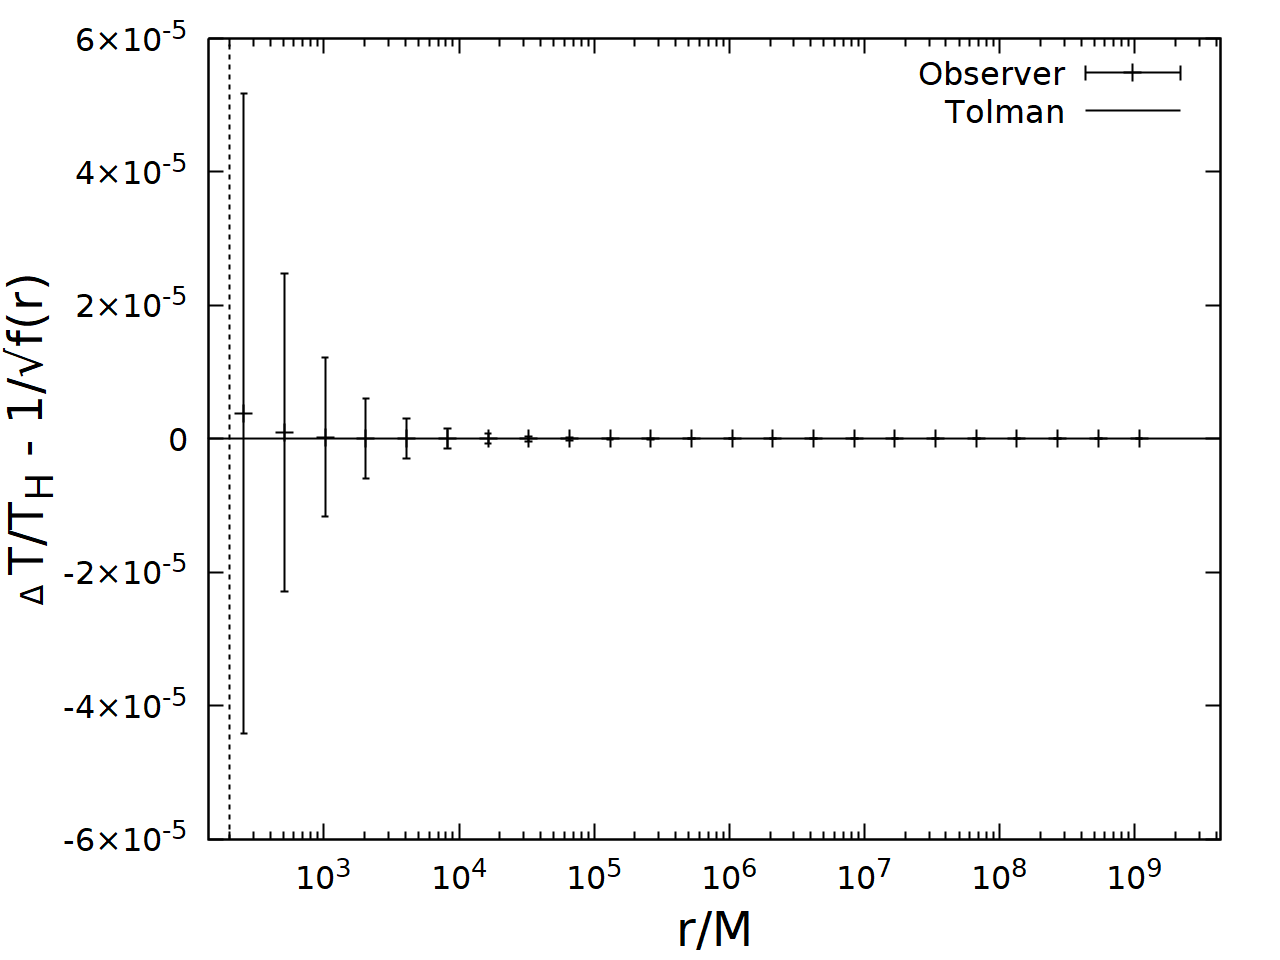
\includegraphics[width=9cm]{../cpp/final/stat_tolman.png}
    \caption{Difference to Tolman relation}
\end{figure}
\end{frame}

\begin{frame}{Circular observer}
\begin{figure}
	\centering
    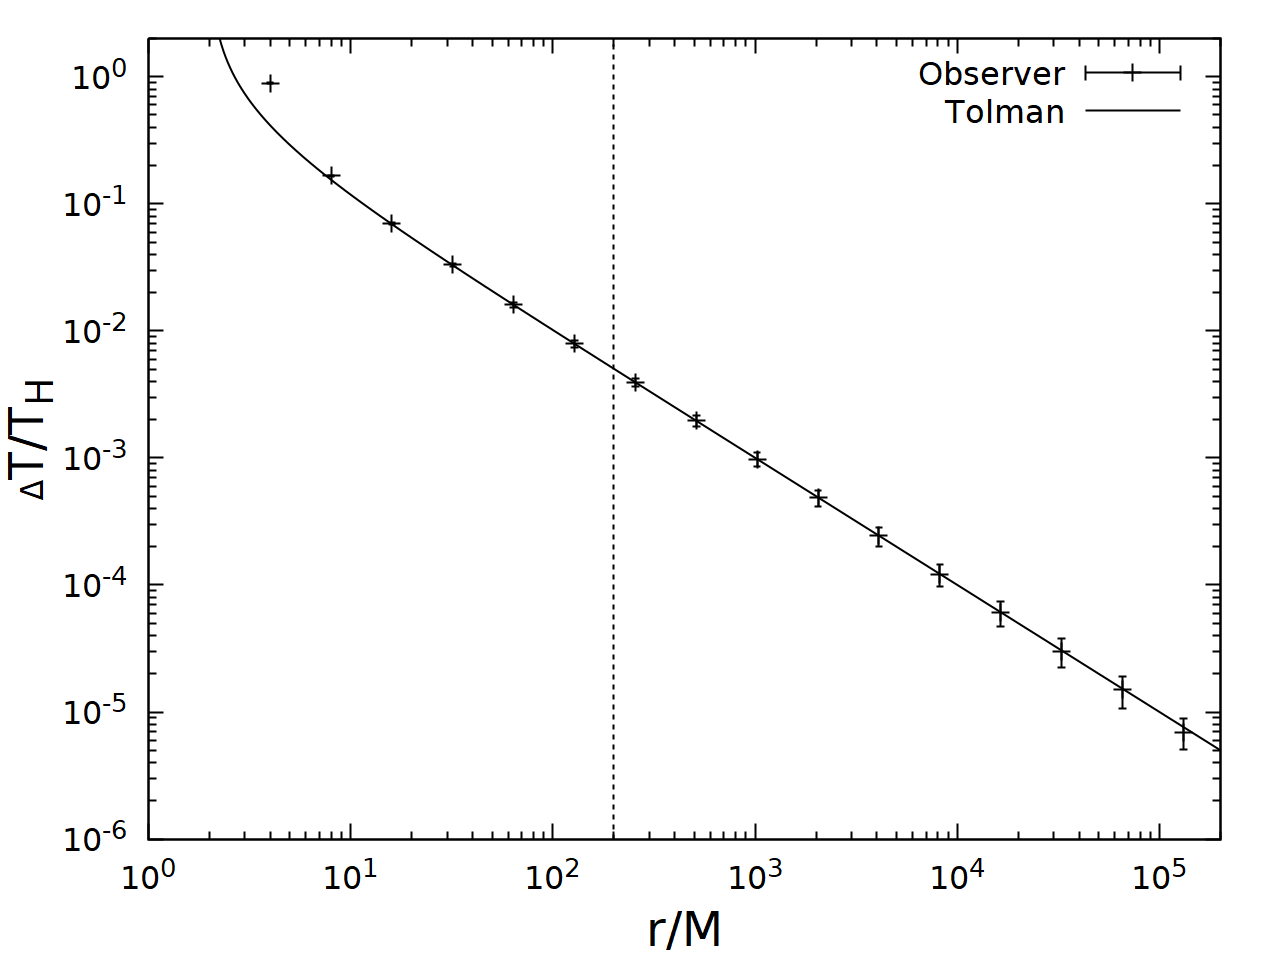
\includegraphics[width=9cm]{../cpp/final/circ.png}
    \caption{Relative temperature shift}
\end{figure}
\end{frame}

\begin{frame}{Circular observer}
\begin{figure}
	\centering
    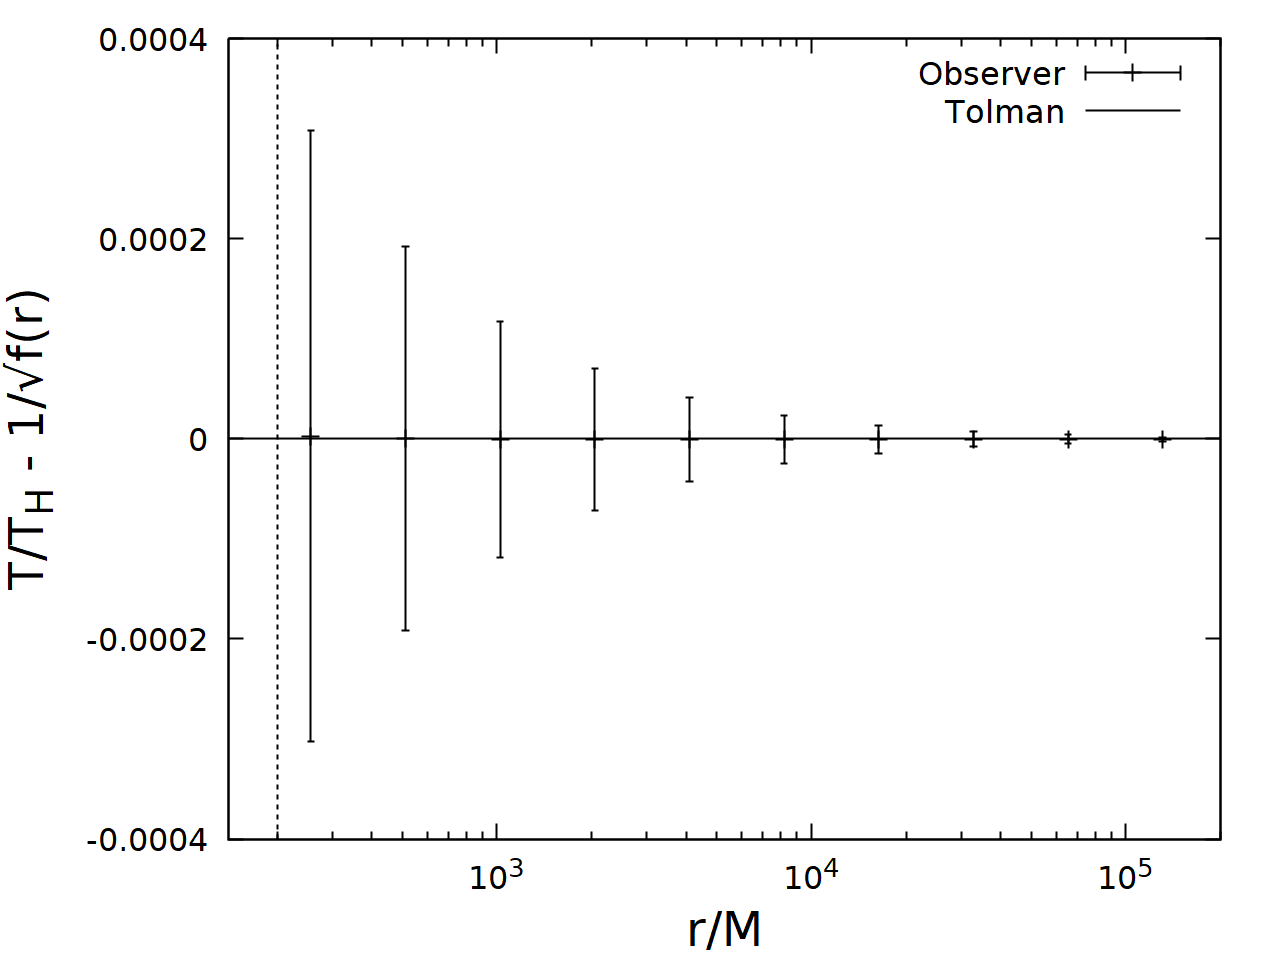
\includegraphics[width=9cm]{../cpp/final/circ_tolman.png}
    \caption{Difference to Tolman relation}
\end{figure}
\end{frame}

\begin{frame}{Infalling radial observer}
\begin{figure}
	\centering
    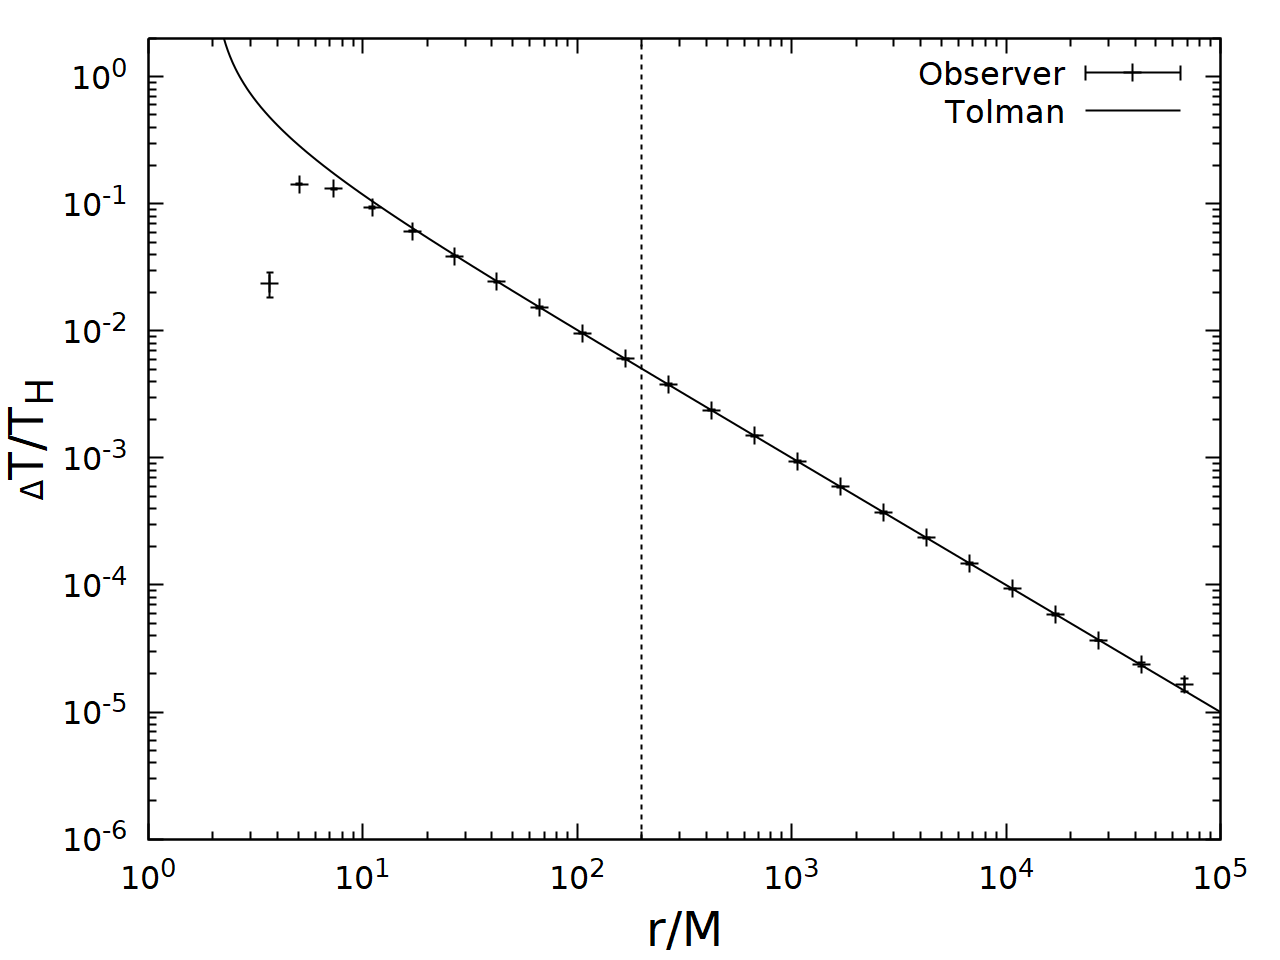
\includegraphics[width=9cm]{../cpp/final/rad.png}
    \caption{Relative temperature shift}
\end{figure}
\end{frame}

\begin{frame}{Infalling radial observer}
\begin{figure}
	\centering
    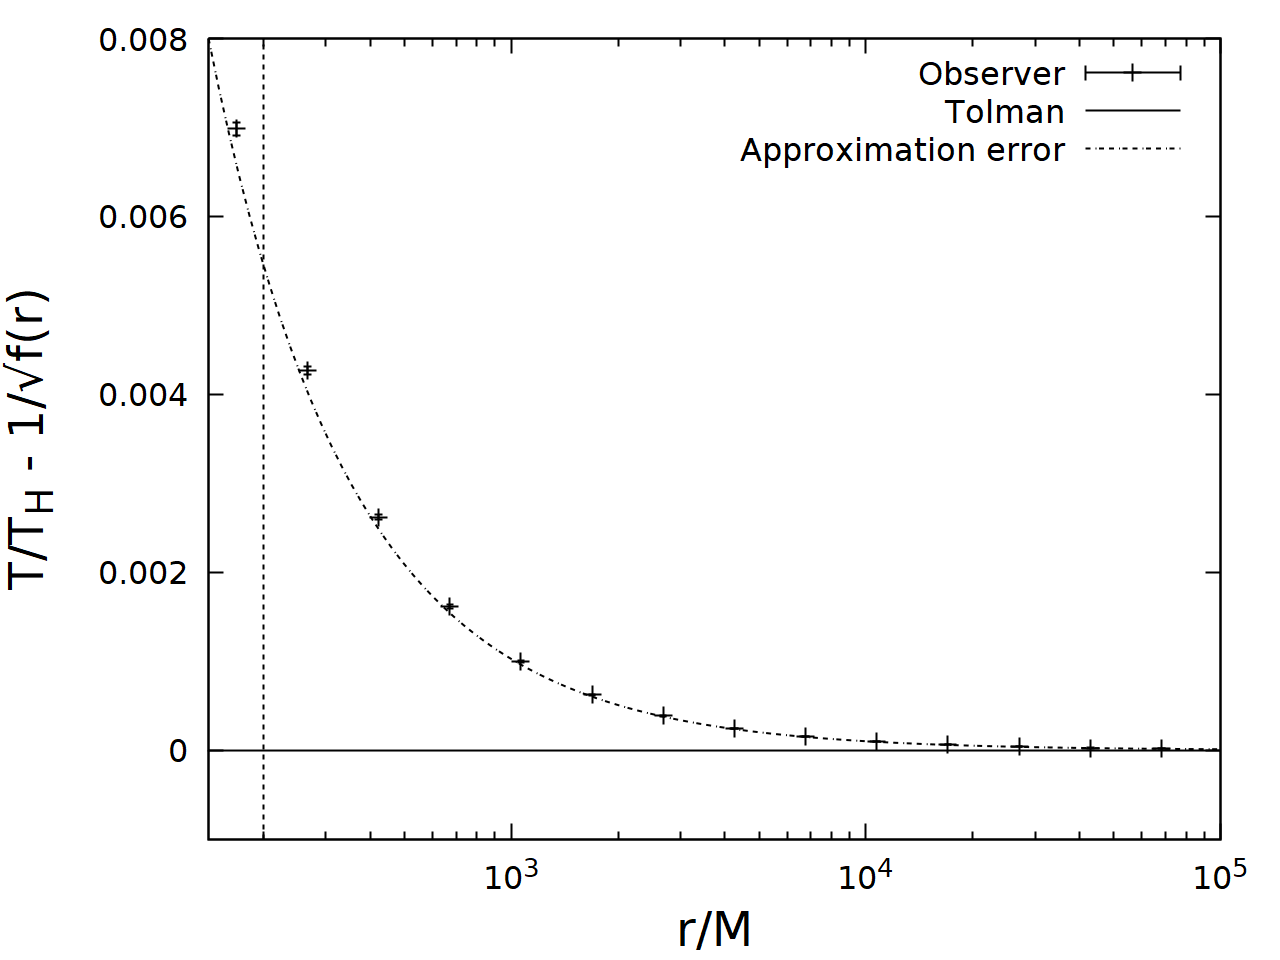
\includegraphics[width=9cm]{../cpp/final/rad_tolman_error_2.png}
    \caption{Difference to Tolman relation}
\end{figure}
\end{frame}

\section{Conclusion}
\begin{frame}{Conclusion}
\begin{itemize}
	\item Equivalence principle not applicable
	\item Approximated \(D^+\) for \(r > 200M\)
	\item Determined the temperature out of a spectrum
	\item For all observers temperature follows Tolman relation
	\item Deviations not significant enough
	\item[\(\to\)] Need better approximation
\end{itemize}
\end{frame}

\begin{frame}{Sources}
\printbibliography
\end{frame}

\begin{frame}
\maketitle
\end{frame}

\begin{frame}{Solutions of Klein-Gordon equation \cite{davies}}
\begin{itemize}
	\item \(u_{\omega l m} = A e^{-i\omega t} \frac{R_{\omega l}}{r}Y_l^m (\theta, \varphi)\)
	\item[]
	\item \(\dv[2]{R_{\omega l}}{r_*} + \omega^2 R_{\omega l} -\qty(\frac{l(l+1)}{r^2} + \frac{f'(r)}{r})f(r) R_{\omega l} = 0\)
	\item[]
	\item Asymptotic: \(R_{\omega l} = e^{\pm i\omega r_*}\)\hspace{3cm}\(r_* = r + 2M \ln \frac{r-2M}{2M}\)
	\item[]	
	\item \(u_{\omega l m} \approx \frac{1}{\sqrt{\pi\omega}} e^{-i\omega t} \frac{\sin(\omega r_* - l\frac{\pi}{2})}{r} Y_l^m (\theta, \varphi)\) 
\end{itemize}
\end{frame}

\begin{frame}{Wightman function}
\begin{itemize}
	\item Wightman function: \(D^+(\vb{x}, \vb{x}') = \int_0^\infty \frac{\dd{\omega}}{\pi\omega} \sum_{l,m} e^{-i\omega(t-t')} \frac{\sin(\omega r_* - l\frac{\pi}{2})}{r} \frac{\sin(\omega r_*' - l\frac{\pi}{2})}{r'} Y_l^m(\theta,\varphi) Y_l^{m*}(\theta',\varphi')\)
	\item[]
	\item Problems:
		\begin{itemize}
			\item IR divergence: \(\int_0^\infty \frac{\dd{\omega}}{\pi\omega} e^{i\omega\dots}\)
			\item[]
			\item Angular dependence: \(\sum_{l,m} Y_l^m(\theta,\varphi) Y_l^{m*}(\theta',\varphi') \sim \delta(\theta-\theta')\delta(\varphi-\varphi')\)
		\end{itemize}
\end{itemize}
\end{frame}

\begin{frame}{Intermezzo: Minkowski space spherical modes}
\begin{itemize}
	\item \(u_{\omega,l,m}\upd{M} = \frac{\sqrt{\omega}}{\sqrt{\pi}} e^{- i \omega t} j_l(\omega r) Y_l^m(\theta,\varphi)\)
	\item Asymptotic: \(u_{\omega,l,m}\upd{M} \to \frac{1}{\sqrt{\pi\omega}} e^{- i \omega t} \frac{\sin(\omega r - l\frac{\pi}{2})}{r} Y_l^m(\theta,\varphi)\)
	\item Wightman function: \(D^+(\vb{x},\vb{x}')\)
	\(\to \int_0^\infty \frac{\dd{\omega}}{\pi\omega} \sum_{l,m} e^{-i\omega(t-t')} \frac{\sin(\omega r - l\frac{\pi}{2})}{r} \frac{\sin(\omega r' - l\frac{\pi}{2})}{r'} Y_l^m(\theta,\varphi) Y_l^{m*}(\theta',\varphi')\)
\end{itemize}
\begin{figure}
\centering
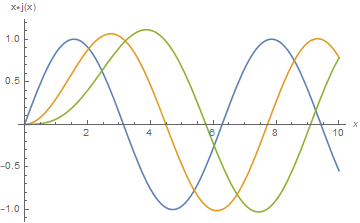
\includegraphics[scale=0.5]{plot/sphericalbessel.png}
\caption{Spherical Bessels: \(x\cdot j_l(x)\)}
\end{figure}
\end{frame}

\begin{frame}
\begin{itemize}
	\item Replace \(\frac{\sin(\omega r_* - l\frac{\pi}{2})}{\omega r} \approx F(r) j_l(\omega r_*)\)
	\item Fix \(F(r)\) for limit \(\vb{x} \to \vb{x}'\)
\end{itemize}
\begin{block}{Wightman function}
	\(D^+(\vb{x}, \vb{x}') \approx -\frac{1}{4\pi^2 \sqrt{f(r)f(r')}} \frac{1}{(t-t'-i\varepsilon)^2 - r_*^2 - r_*'^2 + 2r_*r_*' \cos{\alpha}}\)
\end{block}
\begin{itemize}
	\item Static observer: \(r = \mathrm{const}, \alpha = 0\)
	\begin{itemize}
		\item \(D^+(\vb{x}(\tau), \vb{x}(\tau')) =  -\frac{1}{4\pi^2} \frac{1}{(\tau-\tau'-i\varepsilon)^2}\)
		\item[\(\to\)] No particles
	\end{itemize}
\end{itemize}
\end{frame}

\begin{frame}{Pole at \(\vb{x} = 0\)}
\begin{itemize}
	\item Consider trajectory \(\vb{x}(\tau)\), \(\vb{x}(0) = 0\)
	\item \(D^+\) has second order pole at \(\tau = 0\): \(\frac{1}{a(t(\tau)-i\varepsilon)^2 - |\va{x}(\tau)|^2}\)
	\item \(\varepsilon\) shift pole to upper half:
	\begin{itemize}
		\item \(a(t(\tau_\varepsilon)-i\varepsilon)^2 - |\va{x}(\tau_\varepsilon)|^2 = 0\)
		\item \(\delta\tau = \eval{\dv{\tau_\varepsilon}{\varepsilon}}_{\varepsilon = 0} = ia\dot{t}(0) \pm \sqrt{-a^2 \dot{t}(0)^2 + 1}\)
		\item[] \(\to \delta\tau\) has positive imaginary part
	\end{itemize}
	\item Only poles in the lower half contribute 
	\item[] \(\to\) drop pole at \(\tau = 0\)
\end{itemize}
\begin{figure}
\centering
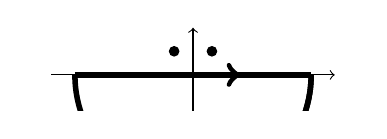
\begin{tikzpicture}[scale=0.3]
  \clip (-7,2) rectangle (7,-1.5);
  \draw[->] (-6,0) -- (6,0);
  \draw[->] (0,-5.5) -- (0,2);
  \draw[line width=2] (-5,0) -- (5,0);
  \draw[line width=2,->] (-5,0) -- (2,0);
  \draw[line width=2] (5,0) arc (0:-180:5);
  \draw[line width=2,->] (5,0) arc (0:-135:5);
  \draw[fill=black] (-0.8,1) circle (0.2);
  \draw[fill=black] (0.8,1) circle (0.2);
  %\draw[thick,<->] (0.5,0.1) -- (0.5,0.9);
  %\node at (0.9,0.5) {$\varepsilon$};
\end{tikzpicture}
\caption{Pole shift}
\end{figure}
\end{frame}

\begin{frame}{Other singularities of \(D^+\)}
\begin{itemize}
	\item \(D^+(\vb{x},\vb{x}') = \bra*{0}\phi(\vb{x})\phi(\vb{x}')\ket*{0}\) satisfies \(\nabla_\mu\nabla^\mu D^+(\vb{x},\vb{x}') = 0\)
	\item[]
	\item Define \(A = 1/D^+ \Rightarrow A \nabla_\mu\nabla^\mu A = 2 \nabla_\mu A \nabla^\mu A\)
	\item[]	
	\item \(D^+ = \infty \Rightarrow A = 0 \Rightarrow \nabla_\mu A\,\nabla^\mu A = 0\)
	\item[] \(\to D^+ = \infty\) is a lightlike hypersurface
	\item[]	
	\item \(D^+\) is singular on lightcone
\end{itemize}
\end{frame}
\begin{frame}
\begin{itemize}
	\item Other singularities appear at \(t = 0\) 
	\item[] \(\to\) no singularities on timelike trajectories 
	\item \(D = [\phi(\vb{x}),\phi(\vb{x}')]\) is only non zero on lightcone
	\item[] \(\to\) \(D^+\) is real for all trajectories 
\end{itemize}
\begin{figure}
\centering
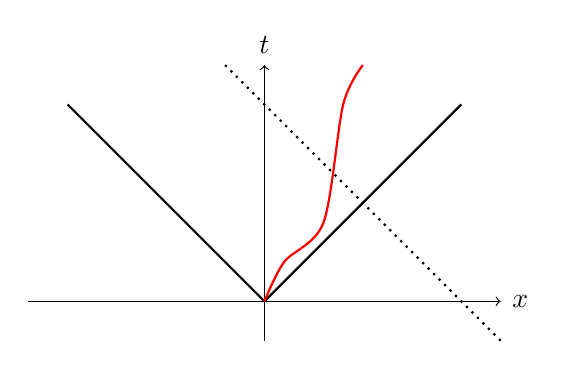
\begin{tikzpicture}[scale=0.5]
  %\clip (-7,2) rectangle (7,-1.5);
  \draw[->] (-6,0) -- (6,0);
  \node at (6.5,0) {$x$};
  \draw[->] (0,-1) -- (0,6);
  \node at (0,6.5) {$t$};
  \draw[thick] (0,0) -- (5,5);
  \draw[thick] (-5,5) -- (0,0);
  \draw[thick,dotted] (-1,6) -- (6,-1);
  \draw[thick,red] plot [smooth] coordinates {(0,0) (0.5,1) (1.5,2) (2,5) (2.5,6)};
\end{tikzpicture}
\caption{Singularities on trajectories}
\end{figure}
\end{frame}

\end{document}